\section{Linear search}
\subsection{Aim}
To perform linear Search in an array of 8-bit numbers.

\subsection{Code}
\begin{lstlisting}
ORG 0000H

MOV R0, #00H ; Resetting R0
MOV DPTR, #0000H ; Starting location of array
MOV R2, #08H ; Count of array
MOV R1, #18H ; Search Element

LOOP:
	MOVX A, @DPTR
	CLR C ; Clear the borrow
	SUBB A, R1
	JZ FOUND
	INC DPTR
	DJNZ R2, LOOP
	JMP EXIT

FOUND:
	MOV R0, #01H

EXIT:
	NOP

END
\end{lstlisting}

\subsection{Output}
\begin{center}
	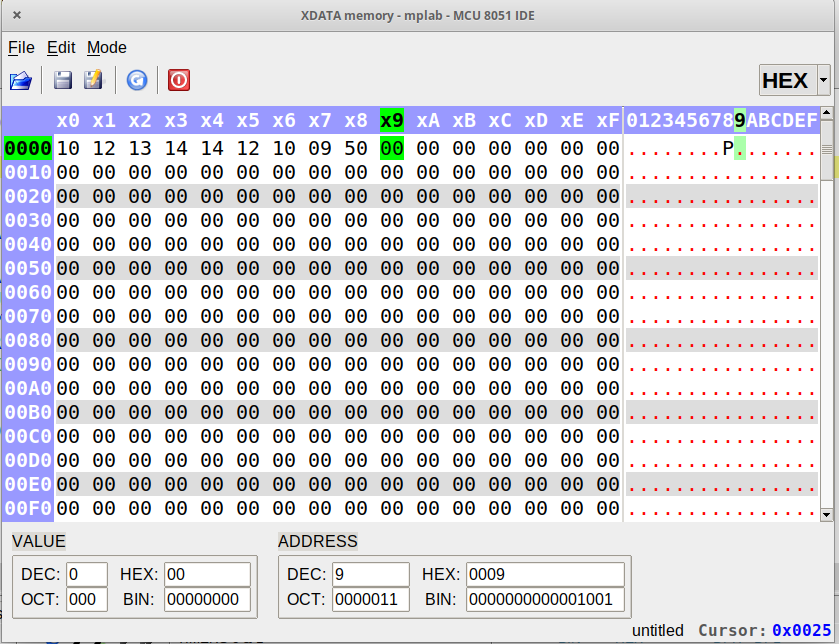
\includegraphics[width=\textwidth]{img/p26/ss1.png}
\end{center}
\textbf{Input} 09H (R1)\\
\textbf{Output} 01 (R0) (Implying the element is found)\\
\begin{center}
	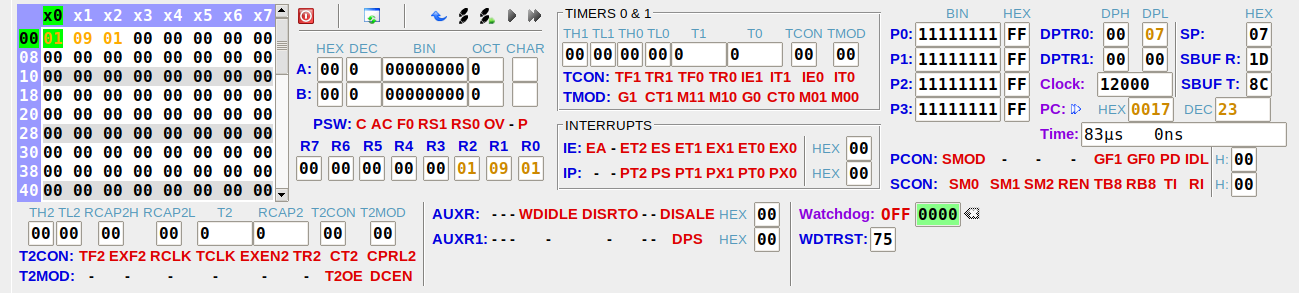
\includegraphics[width=\textwidth]{img/p26/ss2.png}
\end{center}

\textbf{Input} 18H (R1)\\
\textbf{Output} 00 (R0) (Implying the element is not found)\\
\begin{center}
	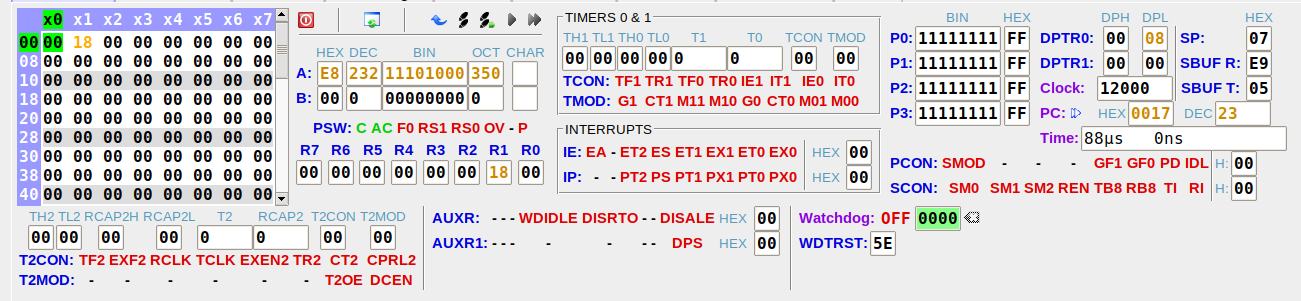
\includegraphics[width=\textwidth]{img/p26/ss3.png}
\end{center}

\subsection{Result}
Linear search was performed in an array in mcu8051ide